\chapter{{\em Silhouette} Execution}
In the previous two chapters,
we identified how and why
multiple executions of the same
Linux service can diverge in behavior.
In light of our results, this chapter introduces a 
novel design strategy that aims to mitigate the bootstorm problem:
{\em silhouette} execution (Section \ref{def:sil}).
For the sake of evaluation, this chapter
presents some design sketches for silhouette
execution for user-mode programs (Section \ref{subsil}).
It also describes the simple simulation techniques we used 
to model the effectiveness of silhouette
execution using our design sketches
(Section \ref{silsimulation}).
From the results of our simulations, we present design ideas
that can improve the effectiveness of
silhouette execution (Section \ref{silimprove})
and evaluate them (Section \ref{sileval}).
Our simulations show that the proposed designs can be successful
in mitigating the bootstorm problem. 

\section{What is {\em Silhouette} execution?} \label{def:sil}
The previous few chapters showed that
distinct executions of the same Linux service
generally execute the same number of instructions
across identical VMs. If the number of booting VMs for
the same physical host is large (as is 
the case in VDI deployments),
then executing many instructions over
and over again during boot represents a waste of scarce CPU cycles.
{\em Silhouette} execution, in essence, targets
redundant execution of the same instructions across distinct but
identical virtual machines in order to reduce CPU pressure in bootstorm
scenarios. 

\newpage
\begin{figure} []
  \centering
  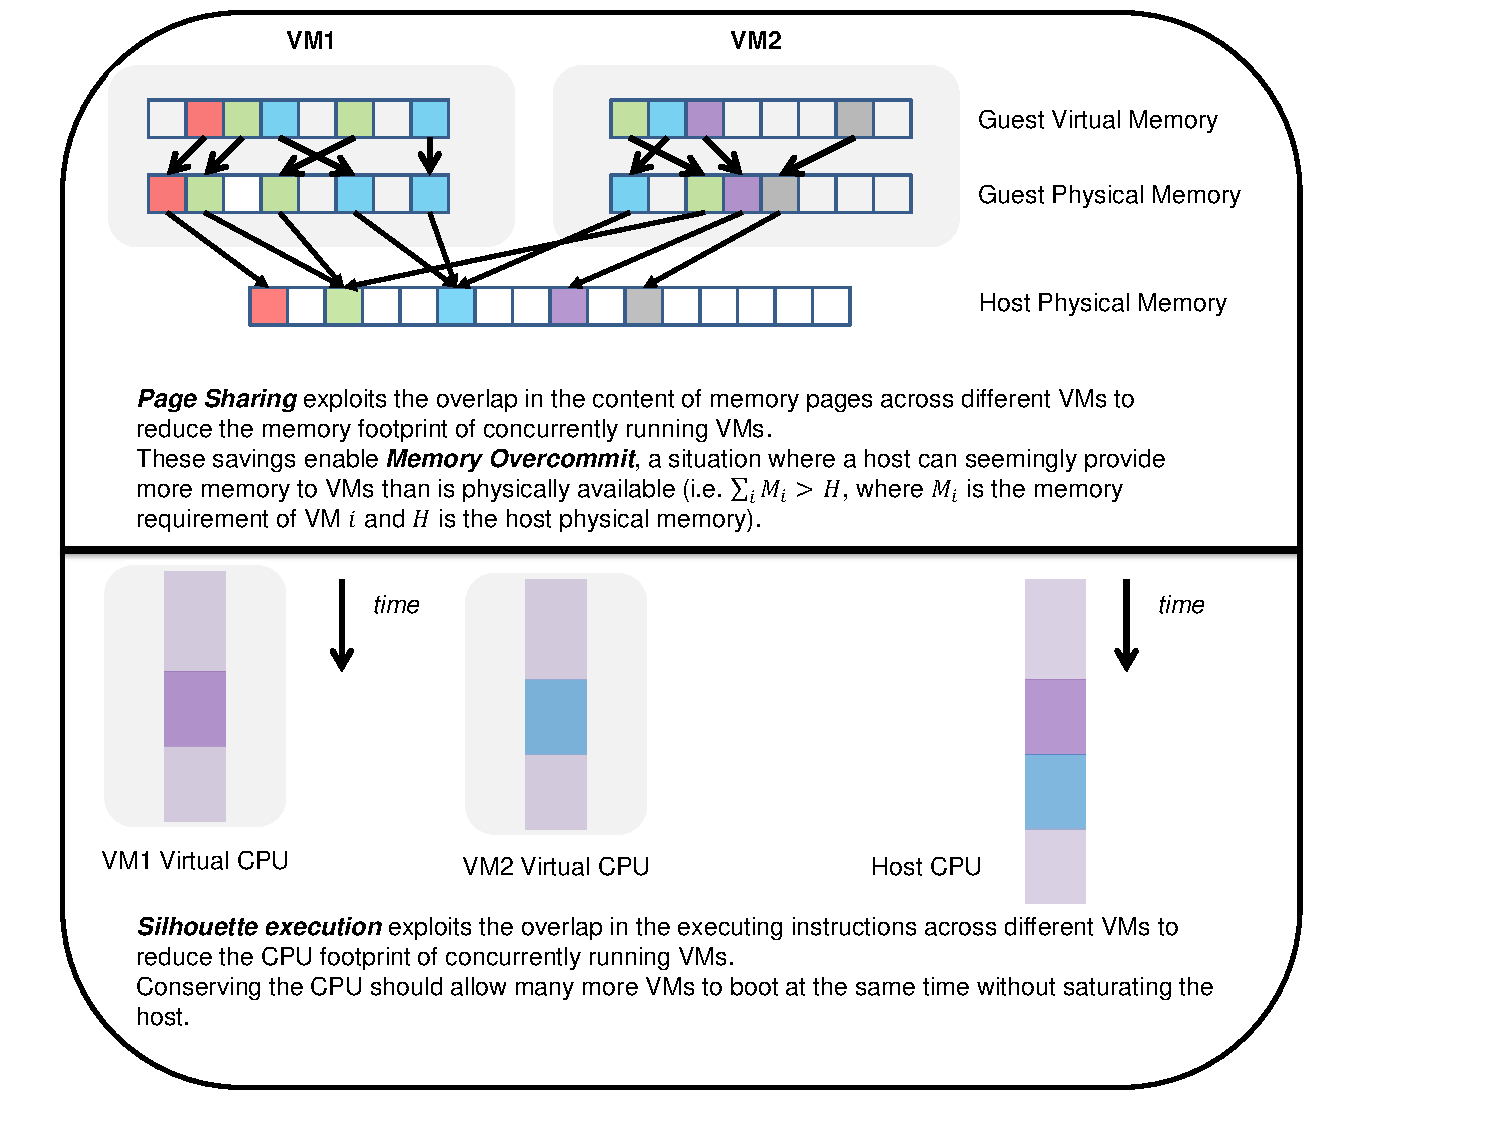
\includegraphics[scale=0.8, trim=2cm 0cm -5cm 0cm]{overcommit.pdf}
  \caption[Silhouette execution is analogous to Page Sharing.]%
          {Silhouette execution is analogous to Page Sharing.}

  \label{silconcept}
\end{figure}

As shown in Figure \ref{silconcept},
silhouette execution is analogous
to page sharing:
both design ideas aim to use hardware
resources effectively to improve VM density per host
in virtualization scenarios.
While page sharing reduces
pressure on the memory subsystem
by identifying and refactoring
overlapping memory contents,
silhouettte execution identifies
overlapping instruction streams
and refactors execution to
reduce pressure on the CPU.
Like memory overcommit,
the ultimate aim is to allow a host 
to support VMs that together require
more hardware resources than are really available
in the host.

To the best of our knowledge, silhouette execution is a novel
design idea that has not been
suggested or implemented before.
To study whether this approach
can be effective in reducing CPU pressure
in concurrently booting VMs,
we evaluate some design sketches for implementing silhouette
execution for Linux services in the rest of this chapter. Admittedly,
user-mode instruction streams 
from Linux services capture
a subset of instructions
executed by a booting VM.
However, we focus on 
Linux services as a first step in
studying the feasibility of 
silhouette execution.
After all, as outlined
Section \ref{linuxboot}, booting VMs
can saturate host CPUs when they launch many
identical user-space processes.
For a complete solution, proposed design sketches need to be 
generalized to the execution of entire
VMs themselves; this would require us to precisely
identify the execution differences that can
arise from all software layers inside a VM. \newline

\section{Silhouette Execution for Linux Services} \label{subsil}
For user-mode Linux services, our
proposed design skeletons for silhouette execution
use  information recorded from one
executing program -- the {\em leader} -- to
bypass execution steps of subsequent instances
of the program  -- the {\em silhouettes}. 
Ideally, the leader executes all instructions from the program, 
while the silhouettes execute a much smaller subset
of these instructions.  

\newpage
To maintain correctness,
silhouettes need only execute: 

\begin{itemize}
\item instructions that can potentially cause the leader's
  execution to differ from the silhouettes (e.g. the \texttt{rdtsc}
  instruction); 
\item instructions that propagate any earlier differences in execution; 
\item instructions that write to memory;
\item system calls that have side-effects to entities
  outside a user-space program
  (e.g. the \texttt{read} system call mutates operating system 
  state associated with file descriptors).
\end{itemize}

If there are no differences between the leader's
execution and a silhouette's, then the silhouette would only
execute the system calls and store instructions
executed by the leader until the login screen is shown.
Executing all the memory writes from the leader
in the silhouettes ensures that the memory image of the two instances
evolves in an identical manner. Executing all the system
calls with the same arguments also ensures
that the silhouette's execution is {\em faithful}
to its semantics, that is, the side-effects to the underlying
operating system are maintained till the end.
Once we restore the register contents
at the end, a silhouette can simply continue
execution independently of the leader.
When the number of system calls and memory read/writes
are much less than all instructions executed,
this approach can, in theory, reduce the stress
placed on the host CPU. 

More generally, when there are instructions
with conflicting side-effects in the leader
and a silhouette, then these instructions
need to be executed by the silhouette as well.
This ensures that the silhouette's execution
semantics are retained. 
It is not known {\em apriori} which instructions in the
two instances of the same program will behave
differently or not.
Our detailed analysis of the various interfaces
between application programs and the operating system
allows us to identify such potential sources of
execution divergence via dynamic 
program inspection.

Note that silhouette execution for user-space programs is fundamentally different
from record-and-replay approaches because it
does not semantically alter subsequent executions
of a program by emulating the leader's execution. 
In fact, silhouettes are independent executions of a program
that can potentially branch from the leader's execution at any point.

The next few subsections outline a few
design sketches for implementing silhouette execution
on individual user-space programs
such as Linux services.
We have not implemented these designs.
Instead, we present them here 
to evaluate the effectiveness of silhouette
execution in user-space.

\subsection{{\em Precise Silhouetting}}\label{precise:sil}
Here is a simple design that uses silhouette execution 
to refactor execution in a user-mode program:

\begin{enumerate}

\item We run one program instance -- the {\em leader} -- 
slightly ahead of all other program instances -- the {\em silhouettes}.

\item Using dynamic inspection techniques on the leader, we
\begin{itemize}
\item precisely identify instructions where other instances of the
program could {\em potentially} diverge. We call these instructions {\em fork-points}.
\item collect an {\em execution signature} that summarizes the 
leader's execution between successive fork-points. For a user-space program, 
this includes a record of memory operations and 
deterministic system calls.
\end{itemize}

\item When a leader reaches a fork-point, it sends its
own execution signature from the previous fork-point (or the
beginning of the program) till the current fork-point to all
other silhouettes. 

\item The silhouettes do not execute
all the instructions that the leader executes.
In fact, each silhouette bypasses execution between
two fork-points by executing only the memory
operations and system calls from the 
execution signature sent by the leader,
and restoring the register state at the end.

\item 
When a silhouette reaches a fork-point, it 
independently executes the {\em forking} instruction
and observes its side-effects.
The forking instruction may or 
may not behave differently
in a silhouette than the leader.

\begin{itemize}
\item If the forking instruction
does have different side-effects
in a silhouette, the silhouette branches execution and 
executes instructions independently
from that point onwards. 
We call this instruction an {\em active} fork-point.

\item Otherwise, we call this instruction a {\em latent} fork-point. 
We return to step 4: the silhouette waits for the leader's
next execution signature for bypassing
execution to the next fork-point.

\end{itemize}
\end{enumerate}

\noindent We name this design {\em precise silhouetting} because
it cannot tolerate any differences in execution
between the multiple instances of a program:
silhouettes completely branch
execution after executing a
forking instruction that disagrees
with the leader (i.e. an active fork-point). 
Our description of precise silhouetting implies
that the leader executes concurrently
with the silhouettes -- albeit slightly ahead --
but this is not necessary.
This approach would work even
if we run the leader to completion
before we run any silhouettes. 
The silhouettes, of course, would only execute system calls and memory
operations between successive fork-points that the leader recorded earlier
until execution diverges.

\subsection{\em Optimistic Silhouetting (excluding control flow)}\label{opt:sil}
{\em Optimistic silhouetting} essentially follows the 
same overall design principles
as precise silhouetting,
except that it allows silhouettes
to tolerate minor execution differences 
before branching execution completely.
In this design:

\begin{enumerate}
\item The leader executes slightly ahead of the silhouettes. 
  The leader identifies fork-points and sends
  execution signatures to silhouettes. 
  The silhouettes bypass execution by only 
  executing the load/store instructions
  and system calls made by the leader,
  and restoring register contents
  at the end of each fork-point.
  This is what happens
  in precise silhouetting before
  the first active fork-point.

\item Unlike the previous design,
  when the leader reaches any fork-point, it always waits
  for the silhouettes to catch up with it.
  All the instances execute a forking instruction
  in sync and compare its side-effects.

\item If a forking 
instruction has different
side-effects in a silhouette
than the leader (i.e. at an
active fork-point): 
\begin{itemize}
  \item the silhouette does not immediately 
  branch execution completely;
  \item the leader tracks the register or 
  memory values that are written differently
  in the multiple instances
  by marking them as {\em tainted};
  \item the leader treats any subsequent instructions that 
  read tainted values as
  fork-points as well;

  \item the silhouettes
  do not overwrite the
  values in any tainted registers
  with those contained in the 
  leader's execution signature.
\end{itemize}

\item When fork-points 
become too frequent, or when
control flow diverges (e.g. a tainted
value is compared to a constant to
determine control flow),
a silhouette starts
executing instructions independently
and branches off from the leader.
\end{enumerate}

\noindent This approach does require that that 
the leader and its silhouettes
execute fork-points at the same time
and communicate their results.
This is necessary so that the leader
can identify subsequent instructions
that propagate any earlier
nondeterminism (e.g. read a tainted
value) as fork points.

\subsection{\em Optimistic Silhouetting (including control flow)}\label{opt:sil}
This design is similar in essence to the version of {\em optimistic silhouetting}  
described above, but it can also tolerate minor control flow
differences between the leader and the silhouettes. 
In this design:

\begin{enumerate}

\item As before, the leader and the
  silhouettes must execute fork-points concurrently. The leader 
  transmits execution signatures to silhouettes, and uses dynamic taint propagation 
  to tolerate minor differences in instruction side-effects.

\item Unlike before, silhouettes do not branch off permanently
  from the leader at the sign of the first control flow divergence:

\begin{itemize}
\item The leader uses dynamic instrumentation to
  create a dynamic {\em control flow graph}
  for the program execution.

\item  When the leader and a silhouette reach a
  control flow fork-point with divergence (e.g. when a tainted value
  is read to determine control flow), the
  leader uses the dynamic control flow
  graph to determine the {\em immediate post-dominator}
  of the block where execution has diverged.

\item   The silhouette branches off
  temporarily (rather than permanently)
  and executes independently to the 
  point of control flow convergence.
  The silhouette and the leader log
  any memory values written 
  or any system calls made
  during this {\em branch interval}.

\item 
  The leader and the silhouette
  compare their current register state, along with the system calls made
  or memory values written during the branch interval. 

\item  An {\em analysis engine} figures out
  whether the two executions are reconcileable
  or not based on what happened
  in the branch interval. 
\end{itemize}

\item 
  If the two executions can be reconciled,
  any conflicting state (e.g memory addresses 
  or register values are
  marked by the leader) as tainted,
  and the silhouettes start
  waiting for execution signatures
  from the leader again.

\item 
  If the two executions cannot be reconciled,
  or when fork-points become too frequent,
  execution branches permanently.
\end{enumerate}

\noindent {\bf Reconciling Executions} \newline
The notion of whether two distinct execution strands 
from a branch interval can be reconciled is a new one.
If two instances do not execute
any system calls or memory operations
during the branch interval, then
execution can be simply reconciled
by marking any different register
values as tainted. If two instances
do execute some memory load/store
operations, then different
memory contents can be marked
as tainted as well to reconcile
them.

If the two instances make different system
calls during the branch interval, then execution may
or may not be reconcilable. 
If the system calls are stateless (e.g. \texttt{time}),
then execution can clearly be reconciled.
On the other hand, if one execution strand
makes system calls that change the operating
system state, then the leader must
know how to identify any subsequent
system calls that depend on the changed state.
For instance, if a silhouette does an
extra \texttt{open} to a
file in the branch interval, the leader
must treat each subsequent \texttt{open}
as a fork point, because
the returned file descriptors
will now be different. The
leader may have previously
assumed that all files to be opened were present
on the identical VMs and thus not
treated the \texttt{open} system call
as a fork-point by default.

There is a clear trade-off in the complexity
in the dynamic instrumentation layer in the leader that tracks
dependencies across system calls and
the extent to which we can 
prolong silhouette execution.
For simplicity, we will assume that
if any instance executes
a system call in its branch interval
that mutates some external state, then the executions
are irreconcileable.

\section{Evaluation Scheme} \label{silsimulation}
The data collection scheme described in Chapter \ref{ch:boot} does not
actually implement silhouette execution in user-space 
because multiple instances execute all application instructions independently.
This section describes how we can still mathematically simulate silhouette execution 
by comparing execution traces from our data collection scheme.

\newpage 
There are several factors
to consider in determining the effectiveness
of silhouette execution.
Ideally, we would like the following
conditions to be true:


\begin{itemize}
\item The first forking instruction
with conflicting side-effects (i.e. the first 
active fork-point) should occur as late as possible 
into the leader's execution.
This is especially important for precise silhouetting,
because silhouettes branch-off
permanently after the first
active fork-point.

\item The number of fork-points should
be much smaller than the total number of instructions executed
by the leader.
All the instances
have to analyze the side effects
of each forking instruction
to determine whether execution has 
diverged or not, which represents 
a serious design overhead.

\item The number of active fork-points
must be small. Fewer 
active fork-points would 
create fewer tainted memory locations,
and thus reduce the overhead
in the leader associated with dynamic
taint propagation.

\item The number of control flow divergences
should be very small. Any control flow divergences
should preferably be short-lived, and have
few system calls or memory operations.
This reduces the overhead
associated with reconciling
executions after branch intervals
and creating dynamic control
flow graphs in the leader.

\item The fork-points must be separated 
by very many instructions so that
memory access logs can be compressed. 
We could forget intermediate
values of memory locations and only
remember their final values instead.

\item Programs should have a high
ratio of user-mode instructions to system-calls
and memory operations so that
silhouettes execute few
instructions compared to
the leader when they are bypassing execution. 

\end{itemize}

\subsection{Computed Metrics}
For our data collection scheme, we can identify fork-points by 
simply parsing the traces collected by our Pin tool
and looking for the sources of potential execution
differences cataloged in the previous chapter. 
Once we can identify individual fork-points, we can compute:
\begin{itemize}
\item The number and distribution of fork-points -- both latent and active -- in a program,
\item The number and distribution of control flow divergences in a program,
\item The proportion of memory and system-call instructions between successive fork-points,
\item Size estimates for execution trace files that need to be communicated between
  the leader and its silhouettes.
\end{itemize}

\noindent Using simple mathematical models, we can compute
the number of user-space instructions the host CPU has to execute
{\em without} silhouette execution ($T_{O}$), and
the number of user-space instructions the host
CPU has to execute under silhouette execution ($T_{S}$)
We measure the advantage conferred by silhouette
execution, $A$, as:
\begin{equation}
A(\vec K, N) = \frac{T_{O}}{T_{S}}.
\end{equation}
$A$ is parameterized by $\vec K = (k1, k2, k3 ...)$
and $N$. $\vec K$ represents the constants
associated with the overhead of various aspects
of silhouette execution and $N$ is
the number of concurrently running instances
of a program.

A value of $A > 1$ implies that silhouette
execution is effective in reducing
CPU overhead from concurrent program execution
on the host in user-space. Generally, $A$ should
increase as $N$ increases (holding everything
else constant), and $A$ should decrease
as individual entries in $\vec K$ increase (holding
everything else constant).
$T_{O}$ is easily computed: $T_{O} = NI$,
where $N$ is the total instances of a program
to be run, and $I$ is the number of instructions
each instance must execute. Typically, $I$ is 
the number of instructions necessary to model
the start of a program or a service. For many Linux
programs, a few iterations of the main
scheduler loop of the program
is sufficiently representative of execution
before a login screen is shown.
The value of $T_{S}$ depends on which version
of silhouette execution is being used. \newline

\noindent {\bf Precise Silhouetting} \newline
Given multiple traces, instructions that are in the common prefix ($P$) 
broadly represent savings from precise silhouetting. Figure \ref{psoverhead} summarizes
how $T_{S}$ and $\vec K$ can be computed
for precise silhouetting. \newline

\begin{figure}
  \centering
  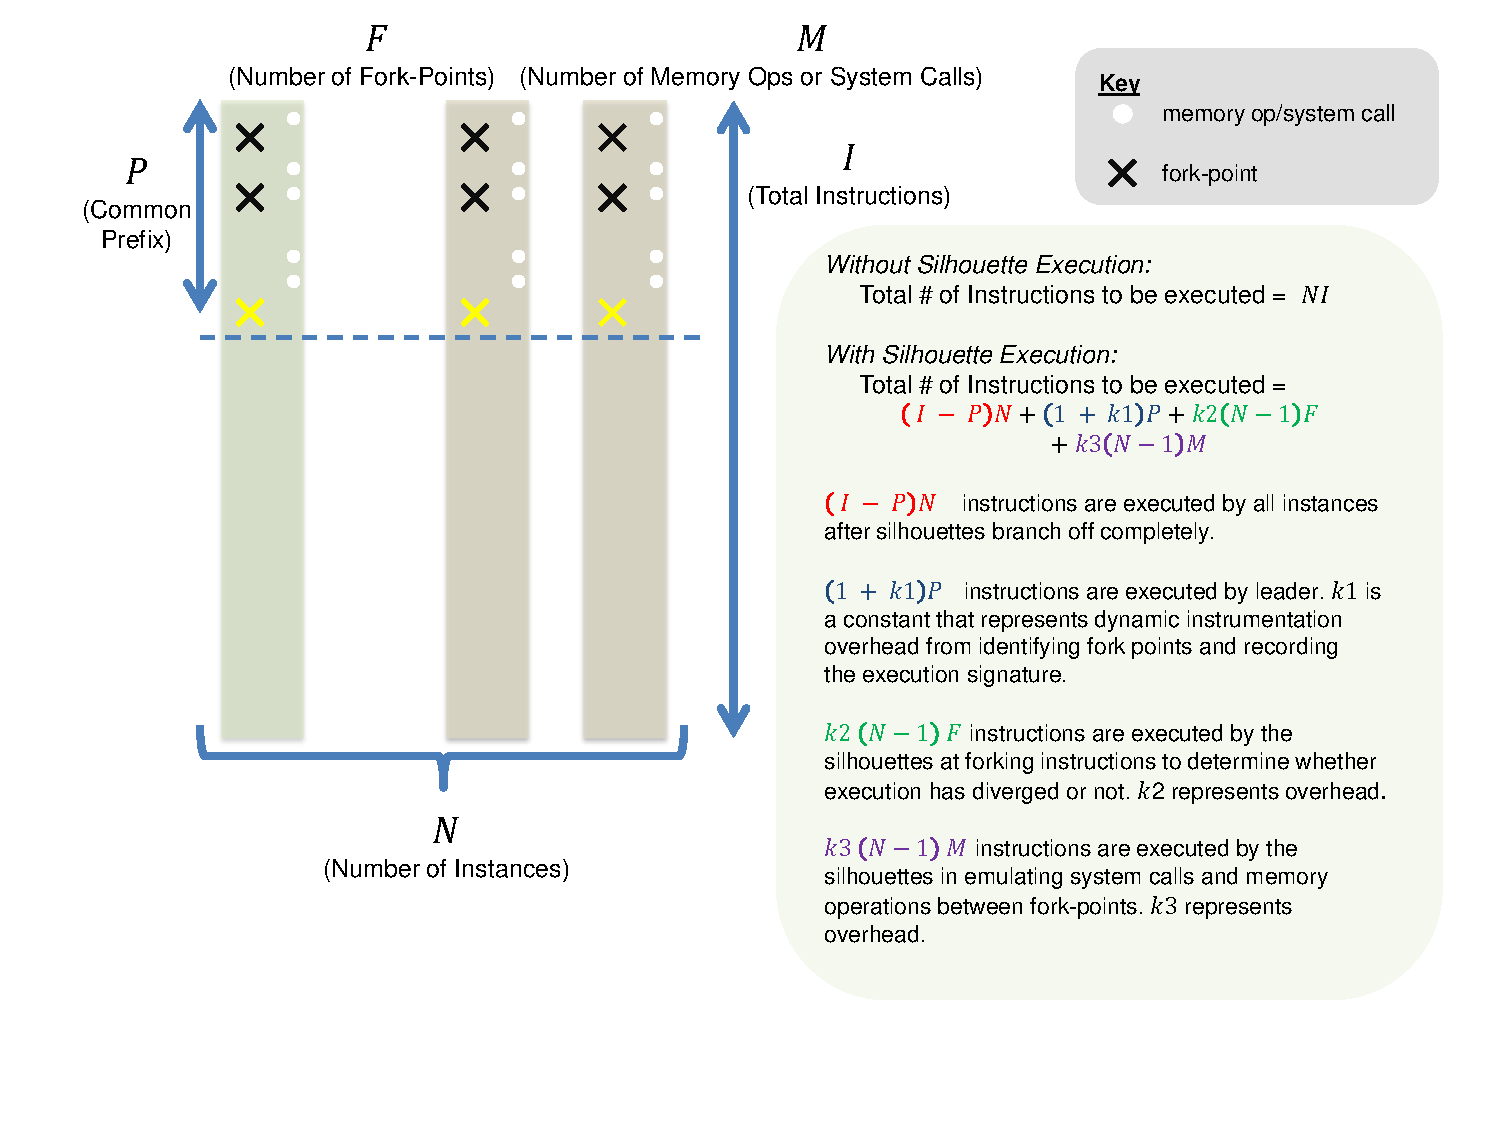
\includegraphics[scale=0.75, trim=3cm 0cm 1cm 0cm]{calc.pdf}
  \caption[Modeling CPU overhead from precise silhouetting]%
          {A simple way to model CPU overhead from precise silhouetting.
            We can compare the user-space instructions executed from running
            a program multiple times in the status quo
            versus the number of instructions executed
            when precise silhouetting is used for
            the same scenario. $k1$, $k2$ and $k3$ 
            are constants that represent overheads
            associated with this approach.}
  \label{psoverhead}
\end{figure}

\noindent {\bf Optimistic Silhouetting (Excluding Control Flow)} \newline 
Instructions in the longest common subsequence ($LCS$)
of multiple traces {\em before} a control flow
divergence broadly represent the savings from 
this variant of optimistic silhouetting.
Figure \ref{osncoverhead} summarizes how $T_{S}$ and $\vec K$ can be computed
for this variant of optimistic silhouetting. \newline

\begin{figure}
  \centering
  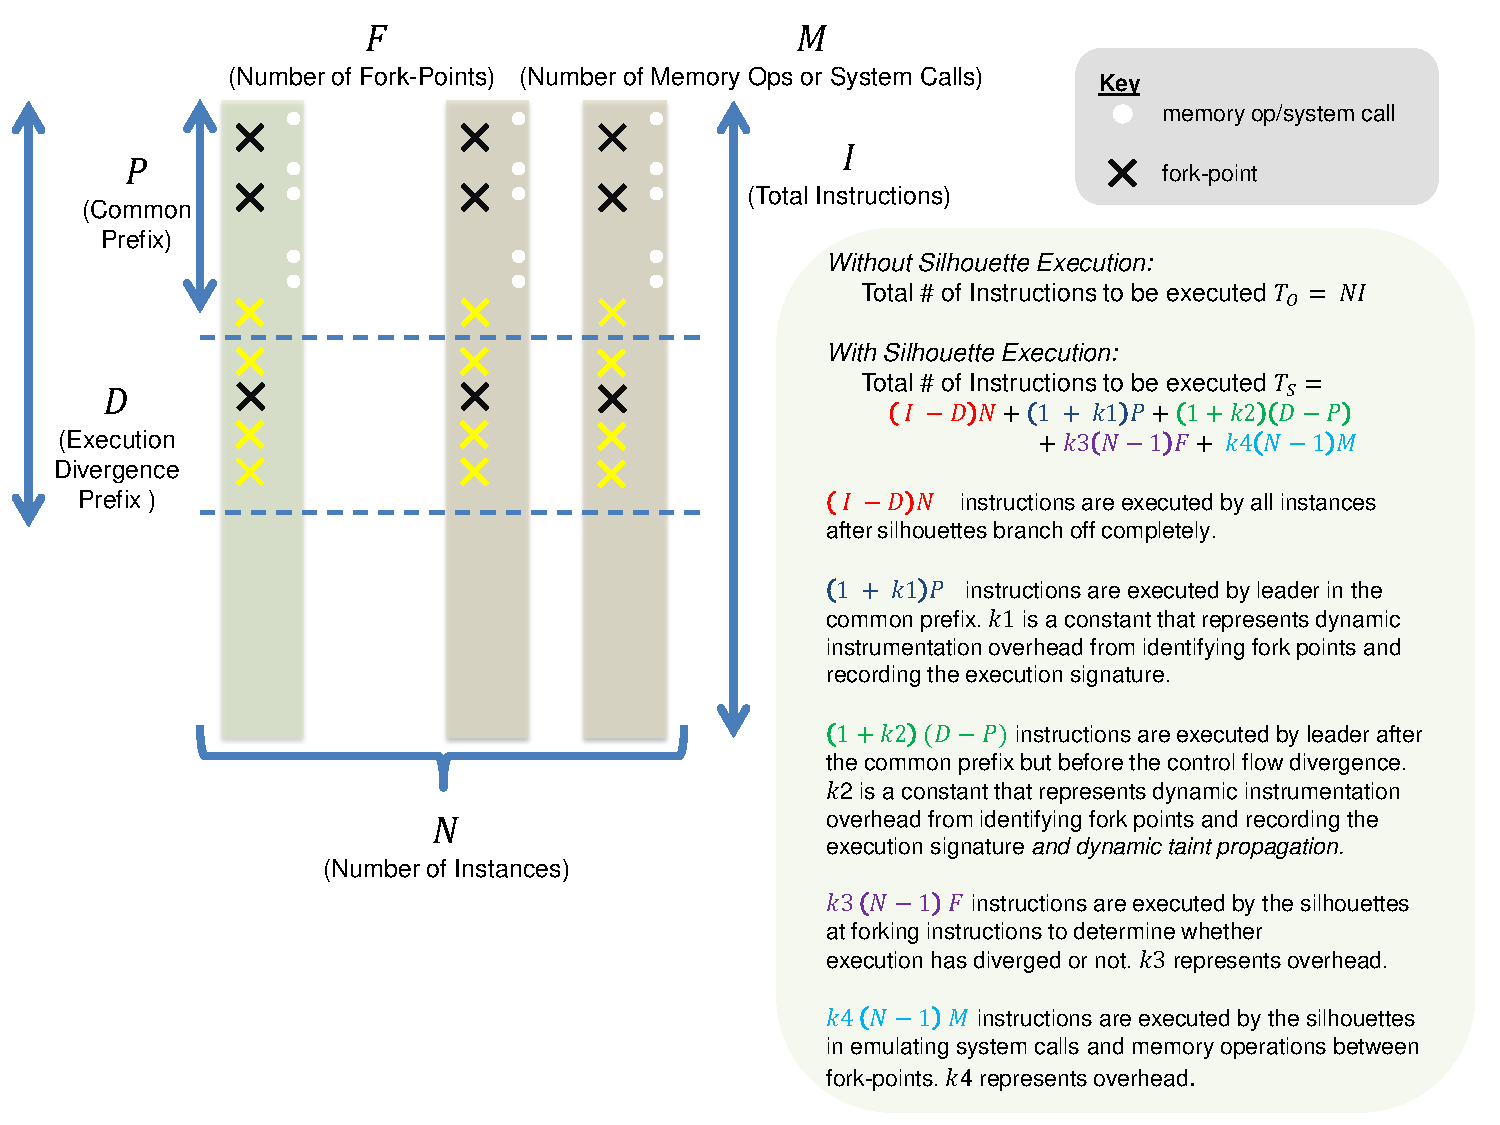
\includegraphics[scale=0.75, trim=3cm 0cm 1cm 0cm]{calc2.pdf}
  \caption[Modeling CPU overhead from optimistic silhouetting (excluding control flow)]%
          {A simple way to model CPU overhead from optimistic silhouetting (excluding control flow).
            We can compare the user-space instructions executed from running
            a program multiple times in the status quo
            versus the number of instructions executed
            when optimistic silhouetting is used for
            the same scenario. $k1$, $k2$, $k3$, and $k4$
            are constants that represent overheads
            associated with this approach.}
  \label{osncoverhead}
\end{figure}

\noindent {\bf Optimistic Silhouetting (Including Control Flow)} \newline
Instructions in the longest common subsequence ($LCS$)
of multiple traces before execution
diverges permanently represent the savings from 
this variant of optimistic silhouetting.
Figure \ref{oscoverhead} summarizes
how $T_{S}$ and $\vec K$ can be computed
for this design. 

\begin{figure}
  \centering
  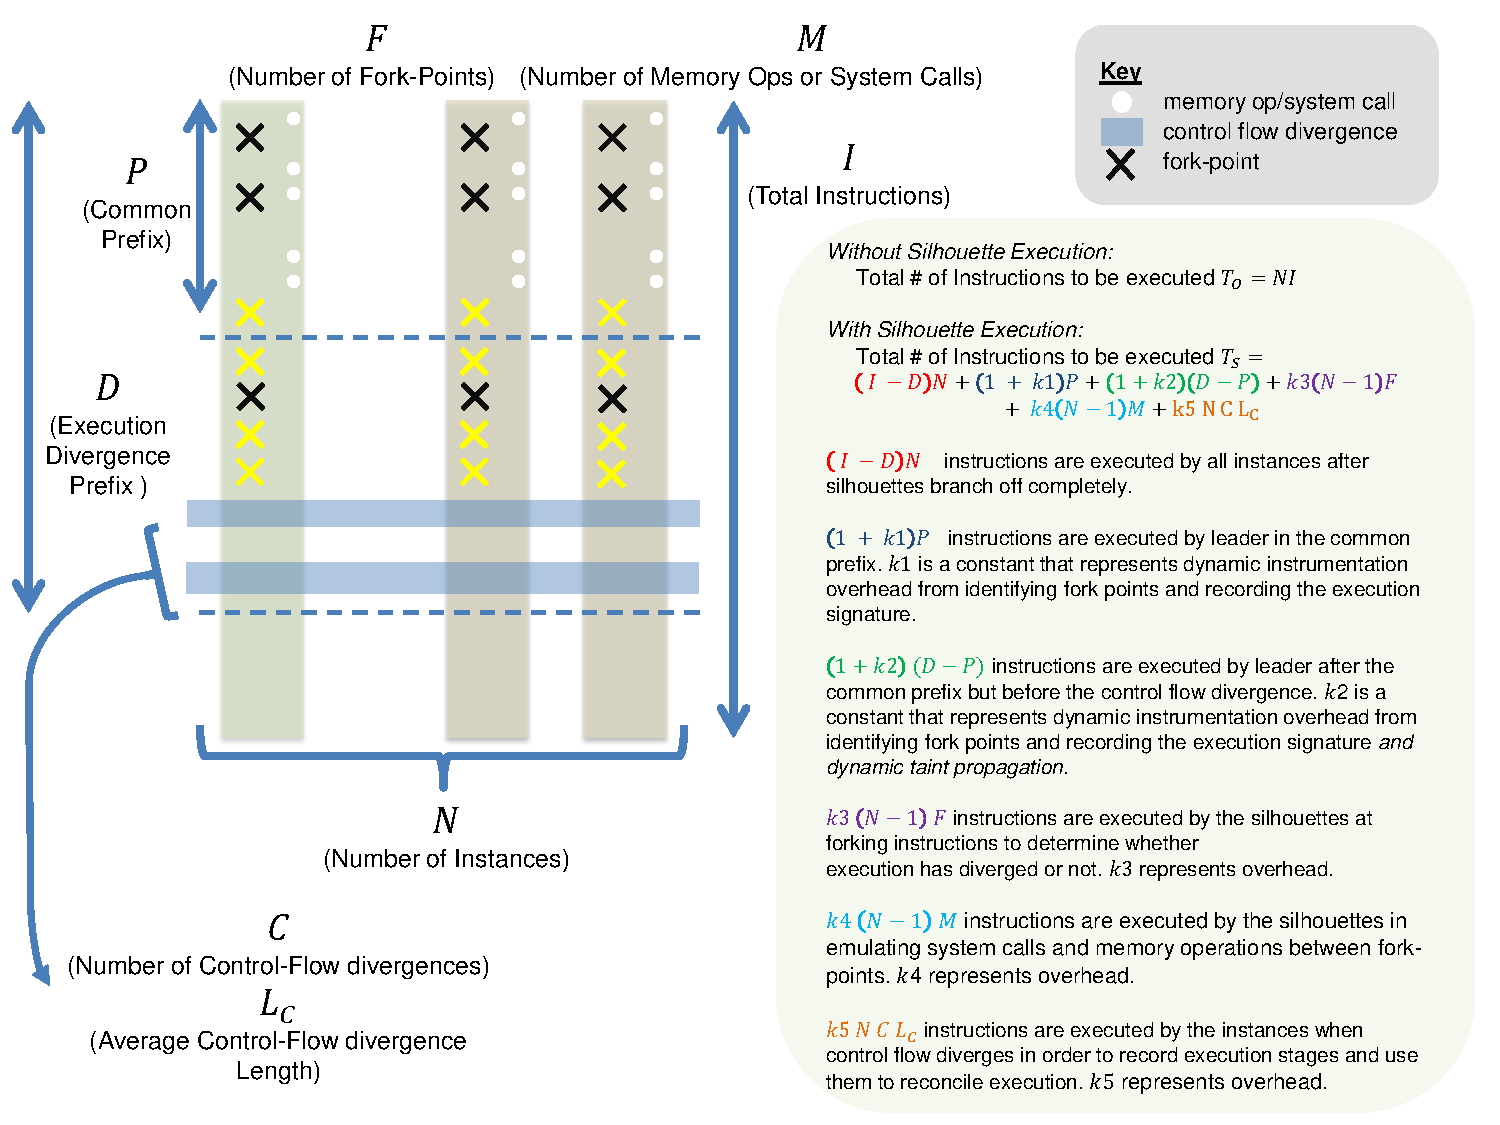
\includegraphics[scale=0.75, trim=3cm 0cm 1cm 0cm]{calc3.pdf}
  \caption[Modeling CPU overhead from optimistic silhouetting (excluding control flow)]%
          {A simple way to model CPU overhead from optimistic silhouetting (including control flow).
            We can compare the user-space instructions executed from running
            a program multiple times in the status quo
            versus the number of instructions executed
            when optimistic silhouetting is used for
            the same scenario. $k1$, $k2$, $k3$, $k4$ and $k5$ 
            are constants that represent overheads
            associated with this approach.}
  \label{oscoverhead}
\end{figure}

\subsection{Caveats}
Before we present our results, we
note a few limitations of our
methods for evaluating 
silhouette execution:

\begin{itemize}
\item We estimate the advantage ($A$) of silhouette execution
on user-space programs purely in terms of the 
number of instructions executed on the host CPU.
We do not model {\em latency} for silhouette
execution. It would be interesting
to study whether the delays introduced
by dynamic inspection of program execution and inter-instance communication
can eclipse the potential latency reduction from reduced CPU load
and bypassing execution in silhouette
execution or not. In practice,
the hypervisor layer 
rather than a dynamic instrumentation layer
would implement silhouette execution,
to reduce performance overhead.

\item Our dynamic instrumentation tool
can only inspect user-mode instructions
of the main process hosting an application,
so we cannot consider code
executed by lower software layers or other
children processes in computing $A$.
Overall, the number of instructions
we consider may be a fraction of all the
instructions computed on the host CPU,
which would add a dampening factor 
to our computed value of $A$.

\item 
The values we use for $\vec K$ are 
conservatively guessed, and
we assume the overheads from various
aspects of silhouette execution are linear in nature.
These assumptions, while reasonable, may understate
the CPU-load reduction practically attainable by silhouette
execution in user-space.

\item We do not factor the storage and I/O overhead
associated with the transmission of execution
signatures, though our experience
suggest that signature files are typically
very small (i.e. only a few megabytes)
so they should fit in host memory.

\item While we collect traces from many different silhouettes,
we simply pick the worst trace (i.e. the one with
the most difference from a leader) for computing
$T_S$. Thus, our models may be overly conservative because they assume that {\em all} 
silhouettes are as different from a leader as the {\em worst} silhouette.
This assumption simplifies the design and evaluation complexity related
from the leader having to handle silhouettes
with varying levels of divergence from
the leader.

\end{itemize}

Despite these limitations, we believe
that our model offers valuable insight
into the feasibility of silhouette execution
in user space because we instrument and evaluate
silhouette execution on large user-mode
instruction streams from Linux services,
and conservatively factor in the possible overhead
from silhouette execution.

\subsection{Initial Results}
\noindent {\bf Precise Silhouetting} \newline
Table \ref{ps:inittbl} shows the results of modeling 
precise silhouetting on a few Linux services.
For simplicity, we include
all system calls in our definition
of fork-points.
This assumption increases the number of fork-points ($F$);
it also increases the overhead associated with determining 
if execution has diverged or not after a fork-point
because the inspection layer has to presumably
understand the logic of each system call
to determine its side effects ($k2$). However,
this assumption reduces $k1$ because an overwhelming majority
of instructions that only use register operands are easily
excluded from fork-points. Instructions
that are system calls are also easily identifiable;
instructions with memory operands need
their memory addresses to be 
compared to tainted addresses (e.g. \texttt{gs:0x14} or \texttt{gs:0x18})
to determine whether they are fork points or not.
For our evaluation, we chose $k1 = 20$,
$k2 = 1000$ and $k3 = 20$ as reasonably
conservative values for the overhead constants.

\begin{table}[h]
  \caption{\hspace{0.2in}Preliminary Results from Modeling Precise Silhouetting \newline \newline 
  $A$, the advantage ratio is calculated by $\frac{T_O}{T_S}$.
  $T_O$ is the total instructions computed in the status-quo whereas $T_S$ is the total instructions computed under
  precise silhouetting. $\vec K$ represents overhead constants; $M$ is the number
  of system calls and memory operations made by the leader before the first active fork-point; $F$
  is the number of latent fork-points before the first active fork-point. $p = P/I$
  the prefix ratio of the execution. }
\label{ps:inittbl}
\begin{center}
\begin{tabular}{|l||c|c||c||c|c|c|c||c||c|}\hline
  Program & $N$ & I & $T_O$ & $p$ & $\vec K$ & $M$ & $F$ & $T_S$ & $A$ \\\hline
  \texttt{cupsd} & 10 & 10000 & 100000 & 0.04\% & (1,2,3) & 499 & 299 & 90000 & 1.11  \\\hline
  \texttt{cupsd} & 10 & 10000 & 100000 & 0.04\% & (1,2,3) & 499 & 299 & 90000 & 1.11  \\\hline
  \texttt{cupsd} & 10 & 10000 & 100000 & 0.04\% & (1,2,3) & 499 & 299 & 90000 & 1.11  \\\hline
  \texttt{cupsd} & 10 & 10000 & 100000 & 0.04\% & (1,2,3) & 499 & 299 & 90000 & 1.11  \\\hline
  \texttt{cupsd} & 10 & 10000 & 100000 & 0.04\% & (1,2,3) & 499 & 299 & 90000 & 1.11  \\\hline

  \texttt{cupsd} & 10 & 10000 & 100000 & 0.04\% & (1,2,3) & 499 & 299 & 90000 & 1.11  \\\hline
\end{tabular}
\end{center}
\end{table}

Because $p$ is very small on average for our sample of Linux services, 
this version of optimistic silhouetting does not offer any savings.
The value of $A$ is 0.40
on average, again representing a {\em degradation}
on CPU load.
 
\noindent {\bf Optimistic Silhouetting (Excluding Control FLow)} \newline
Table \ref{osnc:inittbl} shows the results of modeling 
optimistic silhouetting (without control flow) on our sample of Linux services.
As before, we include all system calls in our definition
of fork-points.
We use the same values of $k1 = 20$, $k3 = 1000$, $k4 = 20$
to model overheads from detection of fork-points in the leader,
execution of forking instructions to distinugish
active and latent fork-points in the silhouettes and
bypassing execution in silhouettes respectively.
We use $k2 = 2k1 = 40$ to model the additional
overhead from taint propagation after the first
divergence.

\begin{table}[h]
  \caption{Preliminary Results from Modeling Optimistic Silhouetting (Excluding Control Flow). \newline \newline 
  $A$, the advantage ratio is calculated by $\frac{T_O}{T_S}$.
  $T_O$ is the total instructions computed in the status-quo whereas $T_S$ is the total instructions computed under
  this variant of optimistic silhouetting. $\vec K$ represents overhead constants; $M$ is the number
  of system calls and memory operations made by the leader before the first active fork-point; $F$
  is the number of latent fork-points before the first active fork-point. $d = D/I$
  the portion of the execution before the first control-flow divergence. }
\label{osnc:inittbl}
\begin{center}
\begin{tabular}{|l||c|c||c||c|c|c|c||c||c|}\hline
  Program & $N$ & I & $T_O$ & $d$ & $\vec K$ & $M$ & $F$ & $T_S$ & $A$ \\\hline
  \texttt{cupsd} & 10 & 10000 & 100000 & 0.04\% & (1,2,3,4) & 499 & 299 & 90000 & 1.11  \\\hline
  \texttt{cupsd} & 10 & 10000 & 100000 & 0.04\% & (1,2,3,4) & 499 & 299 & 90000 & 1.11  \\\hline
  \texttt{cupsd} & 10 & 10000 & 100000 & 0.04\% & (1,2,3,4) & 499 & 299 & 90000 & 1.11  \\\hline
  \texttt{cupsd} & 10 & 10000 & 100000 & 0.04\% & (1,2,3,4) & 499 & 299 & 90000 & 1.11  \\\hline
  \texttt{cupsd} & 10 & 10000 & 100000 & 0.04\% & (1,2,3,4) & 499 & 299 & 90000 & 1.11  \\\hline
\end{tabular}
\end{center}
\end{table}

While $d$ is not as small as $p$
for these Linux services, this version of 
optimistic silhouetting does not offer any savings.
The value of $A$ is 0.50
on average, again representing a {\em degradation}
on CPU load.
This is largely because of a large 
number of fork points and the high overhead
in tracking their side-effects. \newline

\noindent {\bf Optimistic Silhouetting (Including Control FLow)} \newline
Table \ref{osc:inittbl} shows the results of modeling 
optimistic silhouetting (including control flow) on our sample of Linux services.
As before, we include all system calls in our definition
of fork-points. We use the same values of $k1 = 20$, $k2 = 40$, $k3 = 1000$, $k4 = 20$
to model overheads from detection of fork-points in the leader,
taint propagation, execution of forking instructions to distinguish
active and latent fork-points in the silhouettes and
bypassing execution in silhouettes respectively.
We use $k5 = 20$ to model the additional
overhead from execution reconciliation
after a branch interval.

\begin{table}[h]
  \caption{Preliminary Results from Modeling Optimistic Silhouetting (Including Control Flow). \newline \newline 
  $A$, the advantage ratio is calculated by $\frac{T_O}{T_S}$.
  $T_O$ is the total instructions computed in the status-quo whereas $T_S$ is the total instructions computed under
  this variant of precise silhouetting. $\vec K$ represents overhead constants; $M$ is the number
  of system calls and memory operations made by the leader before the first active fork-point; $F$
  is the number of latent fork-points before the first active fork-point;
  $C$ and $L_C$ represent the number of control-flow divergences and their average length
  respectively.  $d = D/I$
  the portion of the execution before permanent execution divergence. }
\label{osc:inittbl}
\begin{center}
\begin{tabular}{|l||c|c||c||c|c|c|c|c|c||c||c|}\hline
  Program & $N$ & I & $T_O$ & $d$ & $\vec K$ & $M$ & $F$ & $C$& $L_C$ &$T_S$ & $A$ \\\hline
  \texttt{cupsd} & 10 & 10000 & 100000 & 0.04\% & (1,2,3,4,5) & 499 & 299 & 4 & 100 & 90000 & 1.11  \\\hline
  \texttt{cupsd} & 10 & 10000 & 100000 & 0.04\% & (1,2,3,4,5) & 499 & 299 & 4 & 100 & 90000 & 1.11  \\\hline
  \texttt{cupsd} & 10 & 10000 & 100000 & 0.04\% & (1,2,3,4,5) & 499 & 299 & 4 & 100 & 90000 & 1.11  \\\hline
  \texttt{cupsd} & 10 & 10000 & 100000 & 0.04\% & (1,2,3,4,5) & 499 & 299 & 4 & 100 & 90000 & 1.11  \\\hline
  \texttt{cupsd} & 10 & 10000 & 100000 & 0.04\% & (1,2,3,4,5) & 499 & 299 & 4 & 100 & 90000 & 1.11  \\\hline
\end{tabular}
\end{center}
\end{table}

While $d$ is larger when we allow for control flow divergences
in these Linux services, this version of 
optimistic silhouetting does not offer any savings.
The value of $A$ is 0.30
on average, again representing a {\em degradation}
on CPU load.
This is again because of a large 
number of fork points and the high overhead
in tracking their side-effects. 

\newpage
\section{Improving Silhouette Execution} \label{silimprove}
When we analyzed the execution
traces collected by our data collection scheme,
we found that several causes of execution
divergence across our sample
of Linux services were synthetic i.e. they were an artefact
of external sources of nondeterminism
rather than semantic differences in program execution.
We thus decided to introduce a determininstic
execution layer to our previous
designs to eliminate as many sources of 
fork-points as possible, to 
improve the feasibility
of silhouette execution.

\subsection{Modified Data Collection Scheme}
We modified our data collection scheme from Chapter \ref{ch:boot} 
(shown in Figure \ref{data:naive}) to simulate and
evaluate silhouette execution in the bootstorm scenario.

\begin{figure}[]
  \center
  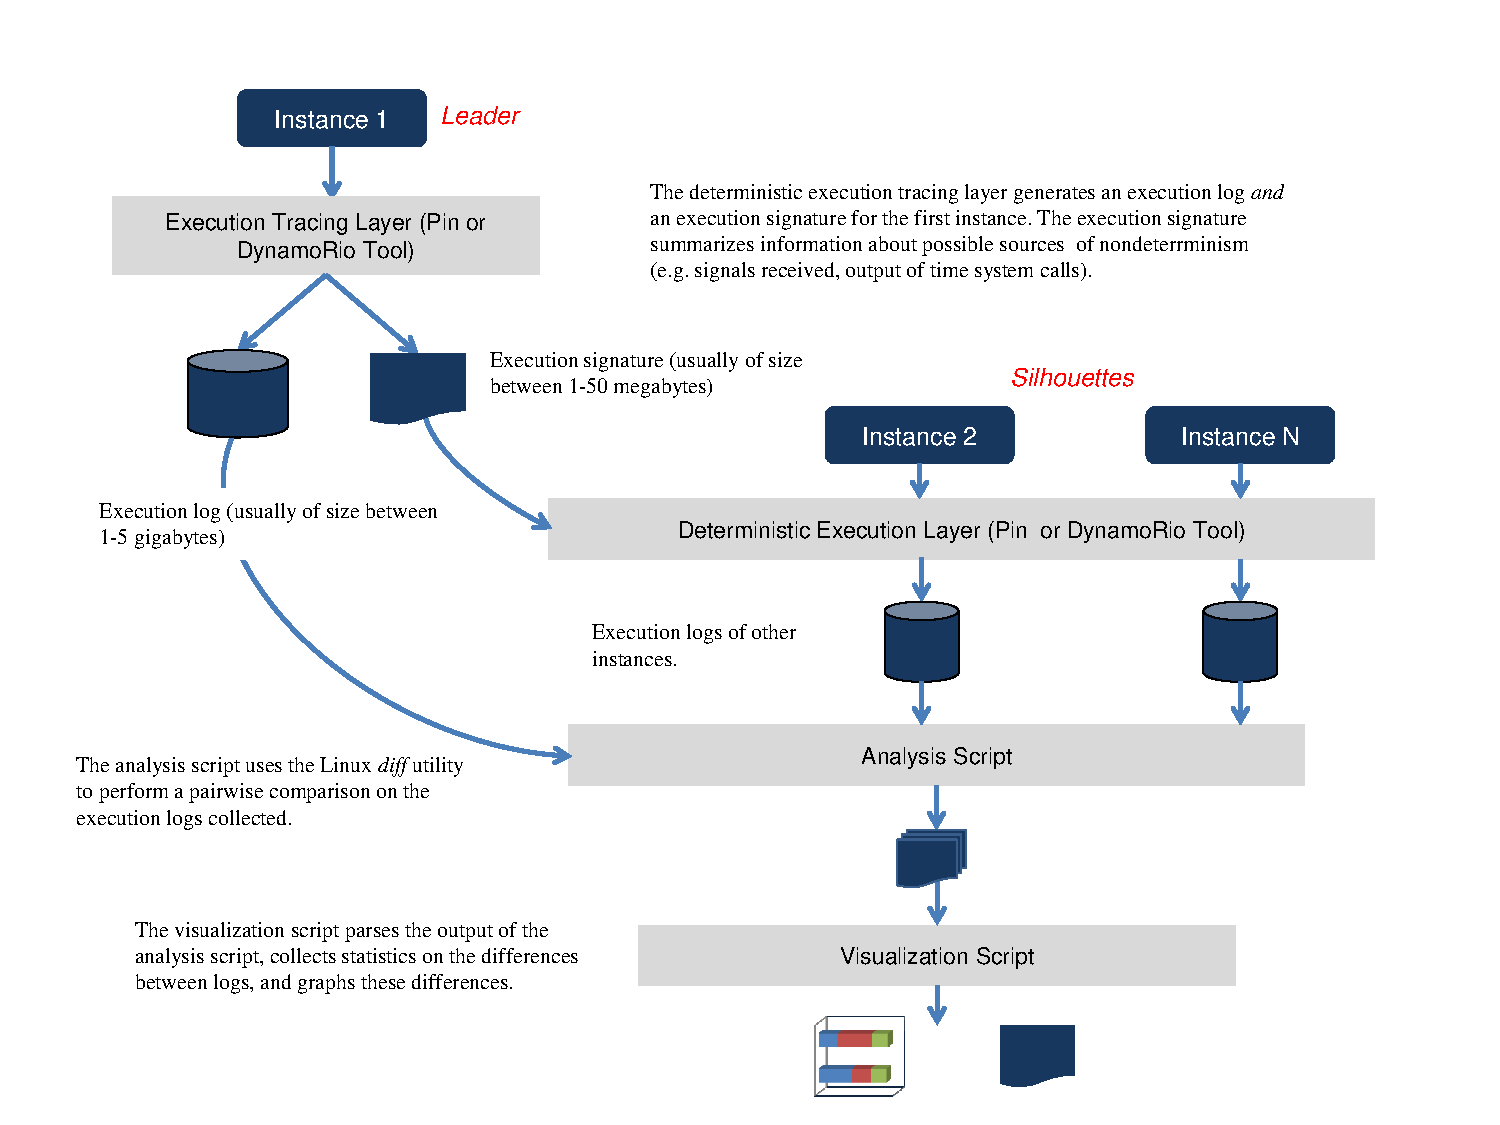
\includegraphics[scale=0.75, trim=2cm 0cm 1cm 0cm]
                  {simulation.pdf}
  \caption[Simulation of {\em Silhouette Execution} in a bootstorm scenario]%
  {Simulation of {\em Silhouette Execution} in a bootstorm scenario.
    We use dynamic instrumentation to 
    generate a trace signature file for the leader.
    While we do not bypass execution in the 
    silhouettes, try to reduce the number of fork-points 
    and record information about them.
    Our analysis and visualization
    scripts allow us to simualate and evaluate
    the effectiveness of {\em silhouette} execution.
  }
  \label{ch3:figsimulation}
\end{figure}


As shown by Figure \ref{ch3:figsimulation}, we run one instance of the
program -- the leader -- before all others.
For the leader, we generate an execution log, as before,
but we also augment the log by summarizing information about the sources of nondeterminism
described in Section \ref{ch3:sources}. For instance, we record
information about signal timing, process IDs, time-related system calls
in the trace signature file. Our Pin tool
uses the trace signature of the leader
to modify the instruction sequences executed by subsequent
executions (the silhouettes) and reduce the number of fork-points
as much as possible.

We run the leader to completion before the silhouettes.
As before, we also do not bypass instructions in silhouettes
so our modified data collection scheme still requires us
to analyze these traces to simulate and evaluate
silhouette execution.

\subsection{Reducing Execution Differences across Instances}
We now describe how dynamic instrumentation can be used to reduce
the source of execution differences from the sources described in \ref{ch3:sources}.
While we modify
the instances that execute after the leader, 
in practice many of our techniques eliminate fork-points altogether 
i.e. the leader can continue execution past
the forking instruction,
or avoid control flow differences by navigating
around variability of I/O timing and latency. \newline

%\noindent {\bf Address Space Layout Randomization (ASLR)} \newline
%Existing record-and-replay systems get around ASLR by
%forcing the operating system to use the same address space layout across
%different runs. A slightly more complex approach 
%would use base/offset computations to translate two equivalent 
%addresses between different executions. 
%For our experiments, we simply disabled ASLR using the command
%\texttt {sudo kernel.randomize\_va\_space=0} to simulate the 
%case where we nudge the operating system to construct
%similar address spaces for the same process. \newline

\noindent {\bf Canary and Pointer Guard Values} \newline
The values of the canary (\texttt{gs:0x14}) and the pointer guard (\texttt{gs:0x18})
are initialized in user-space, so dynamic instrumentation can be used to force 
these values to agree across distinct executions of the same program:
instructions that initialize them can be
modified or replaced or the sources used to compute
these values (e.g. \texttt{rdtsc}, \texttt{`/dev/urandom'}
or \texttt{AT\_RANDOM}) bytes
can be intercepted.

In practice, all this means that a leader can simply choose to
not treat the instructions that initialize \texttt{gs:0x14} or
\texttt{gs:0x18} as fork-points and simply
continue executing past them. The silhouettes will follow the 
leader's execution signature and store the same canary or pointer guard
as the leader into memory. All subsequent instructions
that load the canary or pointer guard values 
from memory will also be identical and thus
can be excluded from fork-points. 
\newline

\noindent {\bf Randomization} \newline
To overcome execution differences resulting from randomization,
we need to intercept the standard techniques
used by programs to seed PRNGs.
In our simulations, values read by the leader from \texttt{`/dev/urandom'}, the
\texttt{AT\_RANDOM} bytes, or the \texttt{rdtsc} instruction 
can be intercepted and recorded in the trace execution file using
dynamic instrumentation in our simulation;
for other subsequent instances, we simply
intercept and replace the return values to match
those from the leader.

In practice, this means that the leader can simply
exclude \texttt{rdtsc} instructions 
or \texttt{read}s from \texttt{`dev/urandom'}
from fork-points and continue executing past them. 
Semantically, when silhouettes replay 
the leader's memory writes, this simulates
the unlikely but possible case that they
received the same random values as the leader.

We need a slightly different approach in practice for \texttt{AT\_RANDOM} bytes because they
are not initialized in user-space.
Simply excluding reads 
of \texttt{AT\_RANDOM} bytes from fork-points
is not sufficient for correctness:
when execution diverges permanently,
a silhouette may read \texttt{AT\_RANDOM}
bytes again and they will be different 
from those read earlier (which is impossible). 
To solve this minor issue, we can make the leader transmit
its \texttt{AT\_RANDOM} bytes
in its execution signature;
the silhouettes overwrite
their own \texttt{AT\_RANDOM}
bytes with the leader's values
before starting execution.
This eliminates
any fork-points or tainted memory
locations that result
from external
sources of randomization
in programs; while
eliminating such randomization
can change execution
semantics of a Linux service,
we are still simulating a valid
(and possible) execution path
for each silhouette. \newline

\noindent {\bf Time} \newline
In our simulations, 
system calls that return 
some measurement of the 
current time, the CPU or program execution time, or a time interval 
(e.g. \texttt{time} or \texttt{gettimeofday})
can be intercepted in the same manner
as randomization:
the timestamps logged
in the trace signature file
can be used to force agreement
between different instances.

In practice, this means that a leader can simply
exclude these system calls from fork-points
and silhouettes copy
the behavior of the leader: this
simulates the unlikely 
but semantically valid scenario
that the various instances
executed the time-related system calls
precisely at the same times.

The timestamps returned from
\texttt{stat} system calls
are not as straightforward
to handle. {\em If} we assume
that all the input, configuration
and data files are identical
between various instances of
a program, then we can 
simply exclude \texttt{stat}
system calls from fork-points.
A leader can assume
by default that various timestamps
returned by \texttt{stat} will
be different and mark
them as tainted.
In our experiences,
the timestamps are typically
ignored in an overwhelming 
majority of cases. Thus, 
tainting these values by
default creates little overhead
because these values are seldom
read or propagated. At the same time,
we avoid the overhead associated
with treating \texttt{stat}
system calls as fork-points.

In the rare cases where
the timestamps from \texttt{stat}
system calls are actually read,
they are typically compared to
determine ``freshness''
(i.e. while file is newer).
When we assume that all
the files accessed by a program
have similar initial contents,
these comparisons can also
be excluded from 
fork-points because timestamps
retain the same order across different
instances of a program
in our experiments. 
Alternatively, when tainted
\texttt{stat} timestamps are compared,
the leader could treat the read as a fork-point
and reexecute the \texttt{stat} system
calls in silhouettes and verify that
the results are the same. In either case, this is clearly a risky
optimization and must be used with care. \newline

\noindent {\bf Signal Delivery} \newline
In order to overcome the unpredictable timing and 
order of signals in our simulations, we intercept all signals received by 
an application and ensure they are delivered
at precisely the same instruction counts
and in the same order as that indicated
in the trace signature file.

Unlike record-and-replay systems, we only
deliver signals that are {\em actually}
received. Thus, signals that are received earlier
than expected are simply delayed or reordered. If,
however, a signal is not received at the expected
instruction count, our instrumentation tool
simply waits or inserts \texttt{nops} until the 
desired signal is received. If a signal simply
refuses to appear for a long time, execution
must diverge. In our experiments,
this final case does not occur as long
as other sources of nondeterminism are controlled. 

In practice, this means that a leader can treat 
received signals as fork-points (as before),
but rather than diverging in control-flow,
it should let silhouettes catch-up with it
and make them wait for the same signal.
This can prevent control
flow divergences and subsequent fork-points that arise from 
variable signal timing and order.
Of course, if the expected
signal is not received in a silhouette
after a long wait, control flow must inevitably diverge.
\newline

\noindent {\bf Process IDs} \newline
In our simulations, nondeterminism from process IDs
can be controlled by virtualizing the process ID
layer, as shown by Figure \ref{ch3:pidfig}.

\begin{figure}[t]
  \center
  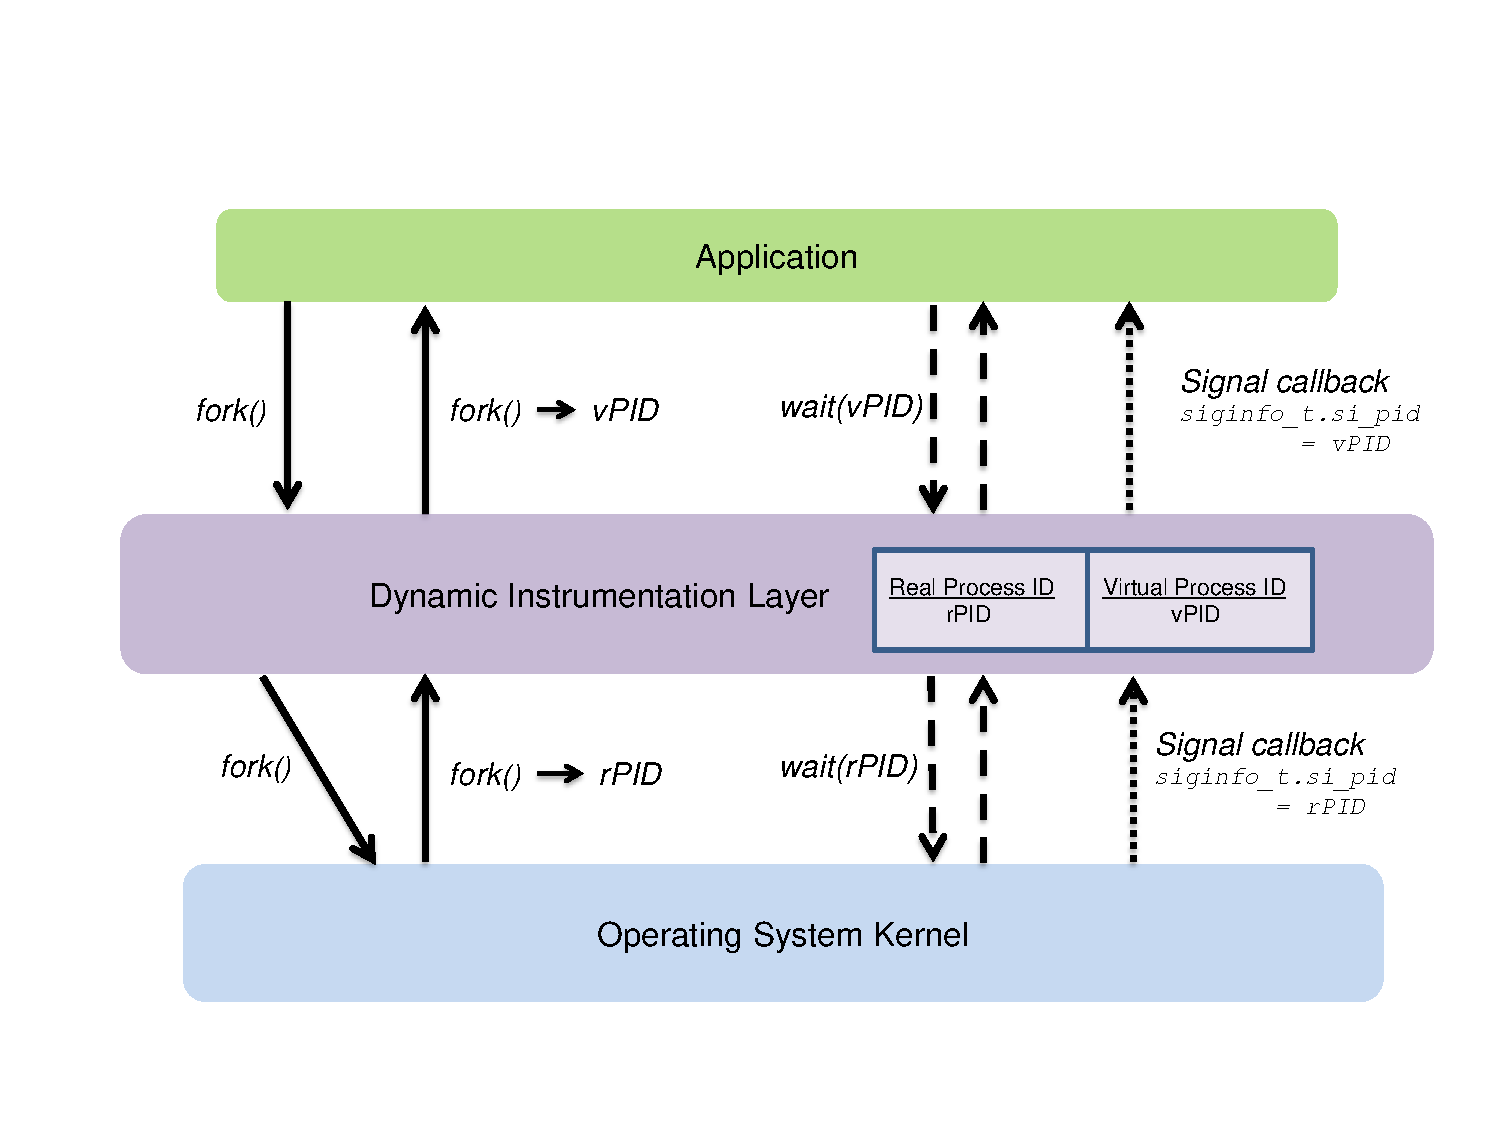
\includegraphics[trim=0cm 1cm 0cm 0.5cm, scale=0.60]{pid.pdf}
  \caption[Virtualizing the process ID layer using Pin]% 
  {All system calls and communications
  between the Linux user and kernel space are intercepted; 
  the dynamic instrumentation layer
  uses a PID translation table, and
  translates between real and virtual process IDs
  to ensure correctness. }
  
  \label{ch3:pidfig}
\end{figure} 

Using dynamic instrumentation, we can replace
real and unpredictable process IDs from kernel space
with virtual and unpredictable process IDs in user space.
As outlined in Section \ref{ch3:pid}, all interfaces
which use process IDs need to be carefully monitored
so that process IDs can be translated back and forth
for correctness. 

In practice, this is equivalent
to using an operating system that assigns
process IDs in a determininstic fashion.



\newline

\noindent {\bf File I/O} \newline
Differences in input file contents across
executions would inevitably cause execution
to diverge, but overcoming nondeterminism arising
from time, randomization or process ID system calls
is typically sufficient to ensure that
file contents rarely differ in Linux services,
if at all. Some files that may differ
between two instances on start up (e.g. 
cache files or logs) can simply be 
deleted or replaced without sacrificing correctness.
Also, as mentioned already, \texttt{stat} 
timestamps are frequently not read, so
they can be replaced with fixed constants;
when they are read and only compared with other
\texttt{stat} timestamps, they can be replaced with 
ordinal numbers that perserve ordering;  
in all other cases, \texttt{stat} system calls 
can be faithfully replayed. \newline

\noindent{\bf Network I/O} \newline
The content of network configuration files
does not change in our experiments, so the strategies 
described to handle \texttt{stat} timestamps 
are sufficient for them. In the same vein, whenever an address is resolved
differently between execution instances because of DNS-based dynamic load balancing, 
we can intercept and replace resolved IPs with those
stored in the execution signature file.

If bytes read from sockets differ across different executions,
we need to understand the {\em context} to determine whether the
differences are serious (e.g. due to different requests)
or synthetic (e.g. due to timestamps). This can
can complicate design of the dynaminc instrumentation
layer because it 
may have to re-execute application or \texttt{libc}
logic to understand differences in raw bytes read from system calls.
We handle nondeterminism from \texttt{Netlink}
sockets in this way: the dynamic instrumentation layer 
re-executes \texttt{libc} logic associated
with understanding contents of \texttt{RTM\_NEWLINK}
messages to detect nondeterminsm from source/destination 
IDs, sequence numbers or interface statistics.
To handle variability in interface statistics,
we can simply overwrite them with fixed values.
This scheme can be generalized to handle
other kinds of network protocols as well.

As an alternative, we could
aggressively intercept Linux socket calls
and blindly replay them in all followers.
When many concurrent executions are reading data from the
same network source, this simulates the possibility
that all instances see the same results over the network
as the first instance. Such an approach, however,
can break correctness (Section \ref{ch3:issues}).
          
\newpage 
To overcome nondeterminism from ephemeral ports, 
we monitor the \texttt{bind} or \texttt{connect} 
system calls and change their arguments to explicitly request ports
in the ephemeral range rather than let the kernel 
assign them; if necessary,
we can also virtualize ephemeral ports
in a similar fashion to how we virtualize process IDs. \newline


\noindent{\bf Scalable I/O Schemes} \newline
To handle nondeterminism caused by unpredictable
ordering of I/O events,
we use techniques similar to those used 
for reordering signals,
as described by Figure \ref{ch3:reorderfig}.

\begin{figure}[h]
  \center
  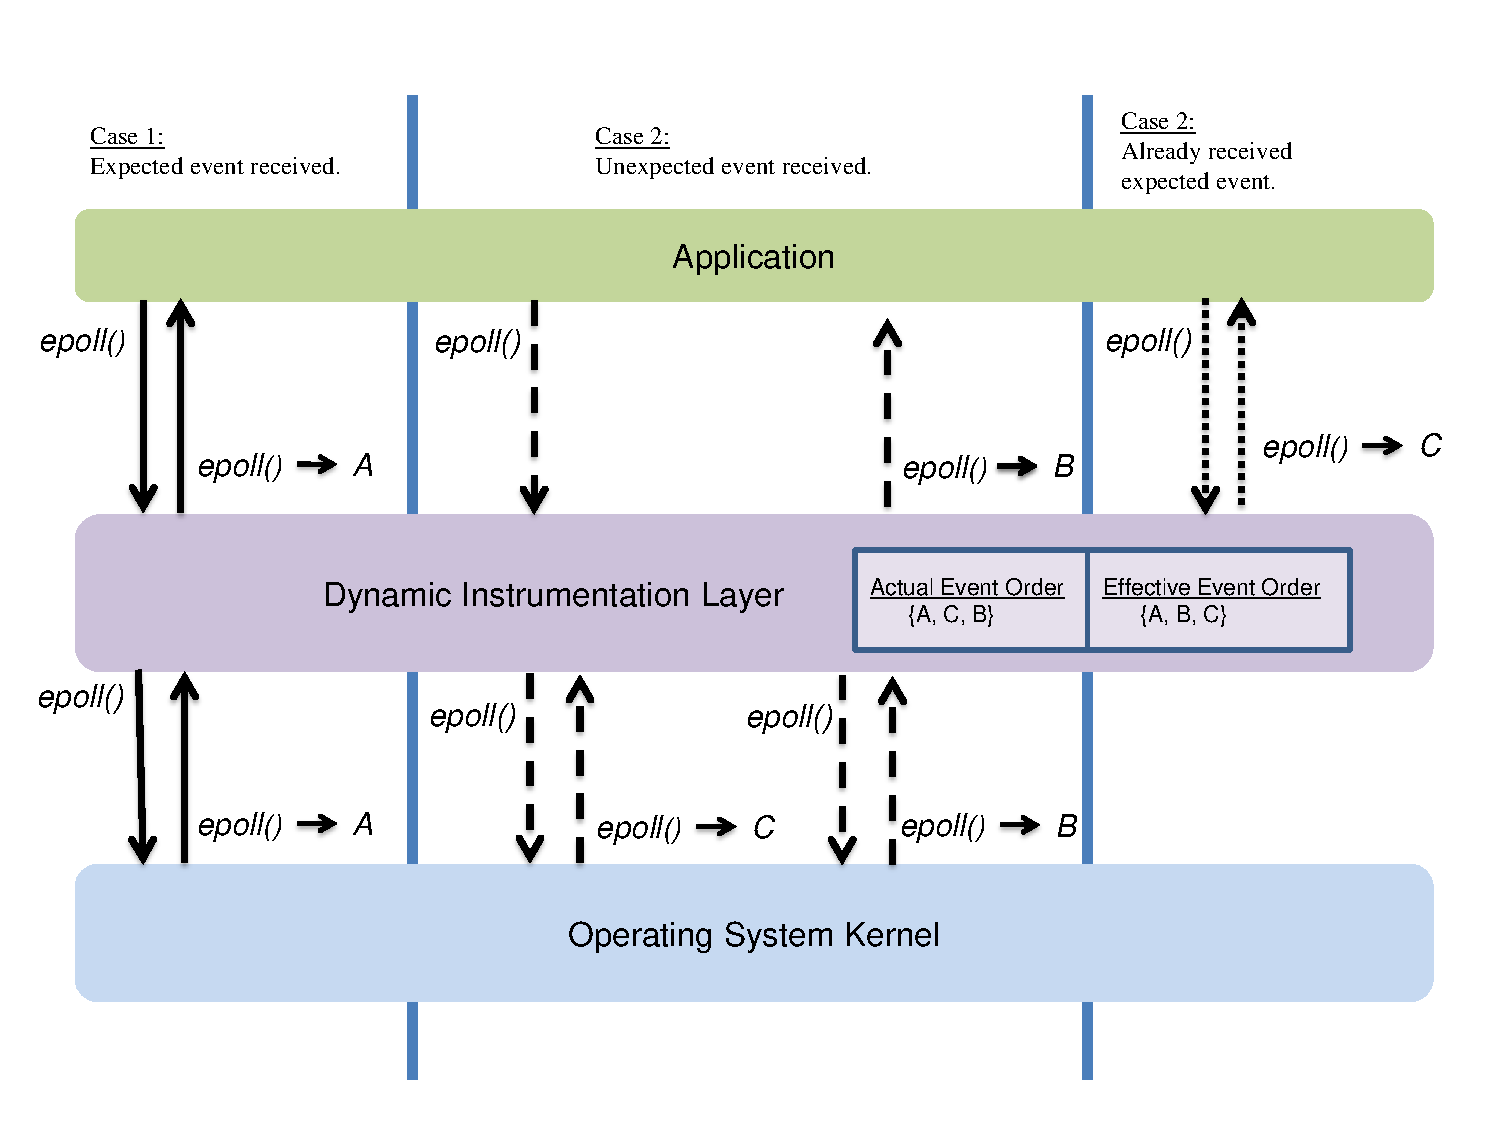
\includegraphics[trim=0cm 1.25cm 0cm 0.75cm, scale=0.60]{epoll.pdf}
  \caption[Reordering I/O events using Pin]% 
    {We intercept all \texttt{epoll} system calls,
    and use the execution signature file to
    achieve determinism. We do not ``replay'' I/O
    events because only events that actually do occur
    are delivered to the application instance. This
    diagram assumes \texttt{epoll} returns one event
    per call for the sake of illustration. }       
  \label{ch3:reorderfig}
\end{figure} 
              
Assuming that \texttt{epoll} returns just one event, figure
\ref{ch3:reorderfig} illustrates three possible cases that could occur:
\begin{itemize}
    \item The event returned by a call to \texttt{epoll} ($A$) is the one expected
    in the execution signature file ($A$). The instrumentation layer
    does not modify the system call.
    \item The desired event ($B$) has not been received yet,
    and \texttt{epoll} returns an unexpected event ($C$).
    The instrumentation layer stores the out-of-order event,
    and repeatedly calls \texttt{epoll} until the 
    the expected event is received.
    \item  A call to \texttt{epoll} is initiated, and the
    event desired ($C$) has already been received.
    The instrumentation layer does not 
    make a system call and simulates a return
    from \texttt{epoll} with the expected event instead.
\end{itemize}

Even if I/O events are reordered,
it is possible that different amounts
of data are available for ready
file descriptors across executions. We can 
mask this effect in the same
way we handle signals: if more bytes
are available (e.g. through \texttt{read}) 
than expected in the execution signature
file, we modify return values and \texttt{read}
buffers to delay the reading of these bytes
until the next \texttt{read}. In some corner
cases, we may have to ``fake'' readiness
in a call to \texttt{epoll}: if all bytes to be read from
a file descriptor have been read by 
the dynamic instrumentation layer (out of which
a few have not yet been delivered to the application),
there will be no more readiness events even
though the application expects them. If less-than-expected
bytes are available, we simply wait
till they are available by waiting for
another readiness update on the same file descriptor inside 
dynamic instrumentation layer.
In our experiments, this approach has been sufficient 
for overcoming nondeterminsm from event-based I/O
schemes.

For asynchronous I/O schemes (e.g. \texttt{aio\_read}), strategies
similar to those used for reordering
and precisely-timing signals would be necessary to hide
variable I/O latency and ordering.
\newline

\noindent {\bf Concurrency} \newline
Nondeterminism due to multi-threading
has been extensively documented; there
is a significant body of work that
attempts to overcome such nondeterminism
by using deterministic logical clocks
or record-and-replay approaches. 
For our experiments, we did not attempt to enforce
a total order on the instructions executed in multi-threaded
programs and just measured nondeterminism inside 
the main process for each Linux service.
To overcome nondeterminism caused
by multi-threading, we could incorporate
deterministic logical clocks 
into our design by augmenting the
execution signature file.

As mentioned before, a nondeterministic system scheduler
can cause variable timing of signals
or I/O events, which
can be handled using reordering and
timing strategies.
Work on deterministic
operating systems can
be extended to overcome this issue
in a more systematic manner. \newline

\noindent {\bf {\em Procfs}: The \texttt{`/proc/directory'}} \newline
Using the techniques described
already, I/O operations on {\em procfs} can be intercepted
and modified. We can 
replay reads from {\em procfs} using the execution signature
file if necessary or replace any statistics with fixed and 
reasonable values. The dynamic instrumentation layer 
must respect differences in virtual and real processes:
it must modify all \texttt{open} system calls with paths
of the form \texttt{`proc/[PID]'}
by switching real and virtual process IDs,
and a process must see its 
parent's virtual process ID when it reads
\texttt{`/proc/[PID]/status'}.

%\section{Results after Using Deterministic Execution} \label{ch3:data}
%We were able to achieve {\em fully} deterministic execution (i.e.
%user-mode execution traces that were 100\% identical) in several
%Linux services including \texttt{cron}, \texttt{ntp} and
%\texttt{cups} using these approaches.

%The next chapter describes the context in which nondeterminism
%occured in these services and the relative
%signficance of the various factors we have outline 
%as sources of nondeterminism in programs.








\section{Evaluation of Simulation} \label{sileval}
In order to evaluate the feasibility of this design,
we need to 
\section {Summary}
